\chapter{Firmware}
\label{ch:firmware}

\section{Análisis}
\label{sec:fw_analisis}

El primer paso para comenzar a trabajar en el firmware del dispositivo es realizar un análisis en el que se concreten los requisitos del sistema.

Como se comentó en la sección \ref{sec:motivacion}, este proyecto es producto de las necesidades de Valeo, una empresa distribuidora de partes de vehículos. Junto a estas, pretenden también proporcionar a sus fabricantes herramientas para probar su correcto funcionamiento. Una de estas herramientas es el PWM Box.

En base a esto, se puede determinar que nuestro producto será usado principalmente en un entorno similar a una fábrica de coches o un taller mecánico. El perfil de su usuario principal será, por lo tanto, el de alguien que no necesariamente tenga conocimientos tecnológicos. Si se espera cierta familiaridad con dispositivos del entorno industrial, con controles similares al nuestro y una interfaz del mismo estilo.

Teniendo en cuenta las necesidades de la empresa y el perfil de este usuario, podemos definir los siguientes requisitos:



\section{Diseño}

Al tratarse de un desarrollo en proceso, el diseño de la arquitectura general del sistema ya estaba realizado. En este aspecto, los cambios a realizar son los derivados de la redistribución del código de algunas partes, que como se determinó en la sección \ref{sec:inginv}, dificultaba la incorporación de nuevas características.

\subsection{Menús}

El principal aspecto a rediseñar está en la parte del sistema que muestra los distintos menús al usuario. La idea es separar la actual implementación de los distintos menús en archivos independientes.

Por un lado, se creará un archivo de control, que será al que se haga referencia desde el resto del programa para hacer operaciones como cambiar de menú, actualizar la pantalla, cambiar el brillo del LCD, etc. Cuando se llamen a funciones que dependan de la pantalla que esté activa en ese momento, él será el que se encargue de delegar la tarea al menú que corresponda.

Por otro lado, cada menú disponible tendrá un archivo separado en el que se implementarán como mínimo las versiones correspondientes de las 3 operaciones básicas (actualizar pantalla, girar \textit{rotary encoder} y pulsar \textit{rotary encoder}). Esto permite que, en menús que requieran funciones específicas (como será el caso del menú de señales lentas que se pretende añadir), estas funciones sólo sean accesibles desde el menú que coresponda.

En la figura \ref{fig:fw_modules} incluída más adelante podemos ver el resultado de esta división. Se destaca también la inclusión de un nuevo tipo de menú, el menú del sistema. Este se encargará de mostrar la secuencia de inicio y el salvapantallas, tareas que estaban antes también unificadas con el resto. También será útil una vez se incluya el almacenamiento de perfiles en la memoria, pues permitirá mostrar un aviso cuando se llene la memoria.

\subsection{Entrada/Salida}

Para la parte de entrada/salida, también se entontraban agrupadas algunas funciones que no estaban del todo relacionadas entre sí. A la vez, se prevee necesario añadir nuevas funcionalidades relacionadas con la comunicación por el puerto serie para integrar el dispositivo con la interfaz gráfica, así como para solucionar los problemas detectados en el \textit{rotary encoder}.

Es por ello que se ha decidido dividir también el código de esta parte en 3 archivos: uno para el puerto serie, otro para el codificador rotarorio, y un tercero para el manejo de eventos.

\subsubsection{Especificaciones acerca de la comunicación por el puerto serie}

Para realizar la comunicación con la interfaz gráfica, se necesitará definir un formato para los mensajes que intercambie esta con el dispositivo.

En primer lugar, conviene determinar de alguna forma el comienzo y el final de un mensaje, lo que nos permitirá evitar errores procesando datos indebidos. Para el comienzo común servirá cualquier carácter que no se vaya a usar en ningún otro punto del mensaje. En este caso, se ha elegido el acento circunflejo (\verb|^|). Para el final, bastará con enviar un retorno de línea (\verb|\n|).

A continuación, se definirá un formato general para los mensajes. Como en este caso se va a realizar la comunicación por el puerto serie, que no es especialmente rápido, se priorizará que los mensajes sean lo más cortos posibles. De esta forma, llegamos a la siguiente especificación:

\begin{center}
    {\fontfamily{cmtt}\selectfont\verb|^T,C(,P1,P2 ... ,Pn)\n|}
\end{center}

Donde:

\begin{itemize}
    \item\textit{T} representa el tipo de mensaje, indicando \textit{?} una petición y \textit{!} un envío de datos.
    \item\textit{C} será una de las siguientes opciones, dependiendo del contenido que se esté transmitiendo:
        \begin{itemize}
            \item\textit{@} servirá como saludo inicial para establecer la conexión entre ambas partes.
            \item\textit{i} para información general del dispositivo.
            \item\textit{c} para la contraseña.
            \item\textit{n} se usará antes de enviar ranuras de memoria, para indicar cuántas.
            \item\textit{s} para ranuras (Slots) de memoria.
            \item\textit{p} para señales PWM.
        \end{itemize}
    \item\textit{Px} serán los distintos parámetros, que dependerán del comando enviado y se encuentran documentados en el código.
% TODO: ¿Añadirlos aquí?
\end{itemize}

Por último, cabría plantear el uso de algún mecanismo de detección de errores. En este caso, dada la baja complejidad y urgencia de la transmisión, se ha optado por posponer este aspecto del diseño, a la espera de probar la comunicación y determinar de forma experimental la frecuencia de errores.

\subsection{Memoria EEPROM}

Para el manejo de la memoria EEPROM, cabe especificar qué datos será necesarios guardar, así como la la forma en la que se van a almacenar los mismos.

En primer lugar se definirán las siguientes unidades:

\begin{itemize}
    \item\textbf{PWM:} Representación de una señal PWM en la memoria. Consistirá de sus 4 parámetros principales (modo, frecuencia, ciclo y fase), así como un nombre identificativo (por ejemplo, "Intermitentes").
    \item\textbf{Slot:} Llamado así por ser la unidad en la que se compartimentalizará la memoria (ranuras), representa una forma de agrupar señales PWM. Permitirá al usuario definir distintos modelos de coches de forma que cada PWM esté destinado a probar un grupo distinto de luces de faros. Consistirá de 8 señales PWM y de un nombre identificativo. Se añadirá, además, una variable que indicará si la ranura está ocupada o no. Esto permitirá evitar borrados reales de memoria, prolongando su vida útil y disminuyendo el coste en cuanto a rendimiento de la escritura.
\end{itemize}

Otros parámetros que se necesitarán guardar son:

\begin{itemize}
    \item\textbf{Valor de inicialización:} Servirá para determinar si la memoria contiene o no datos, ya que en caso de que no los contenga, necesitará ser inicializada con algunos valores por defecto.
    \item\textbf{Número de serie:} Número identificador del dispositivo.
    \item\textbf{Versión del hardware}.
    \item\textbf{Versión del software}.
    \item\textbf{Brillo de la pantalla:} Permitirá mantener el brillo establecido entre ejecuciones.
    \item\textbf{Ranura por defecto:} Indica la ranura de memoria que se cargará automáticamente al iniciar el PWM Box.
\end{itemize}

Según los requisitos establecidos 

Dada la capacidad del usuario de añadir, borrar y reemplazar ranuras de memoria según desee, se prevee la necesidad de algún mecanismo adicional para determinar qué ranuras mostrar en el menú principal del dispositivo. Con este fin, se incluirá también un vector auxiliar, que contendrá el índice de las ranuras de la memoria en el orden en el que se les muestra al usuario. Actúa, por así decirlo, como un traductor entre el índice de las ranuras visibles al usuario y el índice de las mismas internamente. Esto puede entenderse más fácilmente con una representación, que se incluye en la \autoref{fig:eeprom_operations}

\begin{figure}[h]
    \centering
    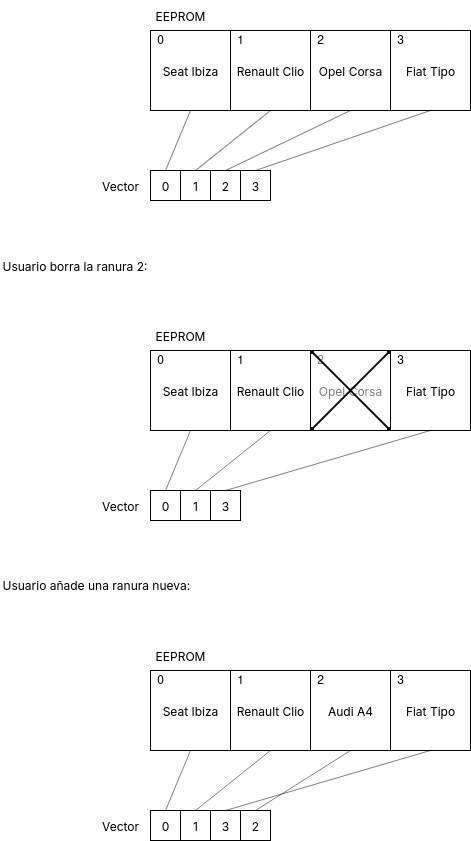
\includegraphics[width=0.8\textwidth]{eeprom_operations.png}
    \caption{Representación del funcionamiento del vector auxiliar al realizar distintas operaciones sobre la EEPROM.}
    \label{fig:eeprom_operations}
\end{figure}

\subsection{General}

La organización de los archivos dentro del proyecto también se considera un aspecto importante a tener en cuenta para facilitar el trabajo. Añadir los archivos comentados en la subsección anterior a los ya existentes en el proyecto no resultaría beneficioso en este aspecto.

Para tratarlo, se plantea cambiar la distribución a la mostrada en la \autoref{fig:fw_modules}.

\begin{figure}[ht]
    \centering
	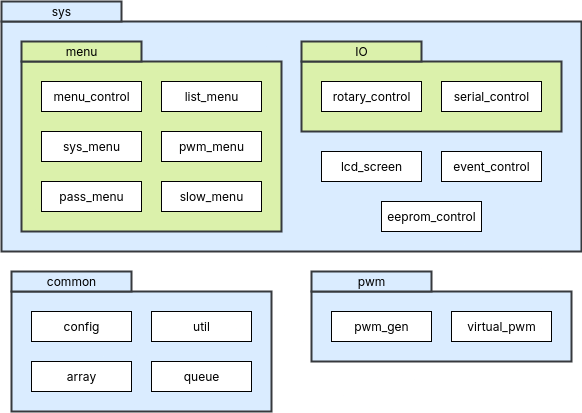
\includegraphics[width=\textwidth]{fw_modules.png}
	\caption{Distribución del código en distintos archivos y módulos.}
    \label{fig:fw_modules}
\end{figure}

En ella, podemos ver los distintos directorios, a los que llamamos módulos, en los que se dividirán los archivos de código. Cada uno de ellos se centrará en un aspecto del firmware. Se distinguen los siguientes:

\begin{itemize}
    \item\textbf{Módulo del sistema:} Contiene la implementación de características claves para el funcionamiento del sistema.
        \begin{itemize}
            \item\textbf{Módulo de E/S:} En él entontramos los archivos que definen el funcionamiento del \textit{rotary encoder} y de la UART, responsables de la comunicación con el usuario y la aplicación respectivamente.
            \item\textbf{Módulo de menús:} Agrupa la implementación de los distintos menús que usa el sistema.
        \end{itemize}
    \item\textbf{Módulo de PWM:} Se encarga de la generación y configuración de las señales de salida.
    \item\textbf{Módulo de archivos comunes:} Se tratan de utilidades genéricas, pensadas para ser usadas en común por las distintas partes del programa.
\end{itemize}

\subsection{Resultado final}

Tras estos cambios, el código queda más agrupado según su funcionalidad. Podemos ver cómo quedaría una ejecución del bucle principal en la representación de la \autoref{fig:fw_loop}. Adicionalmente, la \autoref{fig:fw_interrupts} recoge el manejo de las interrupciones.

\begin{figure}
    \centering
    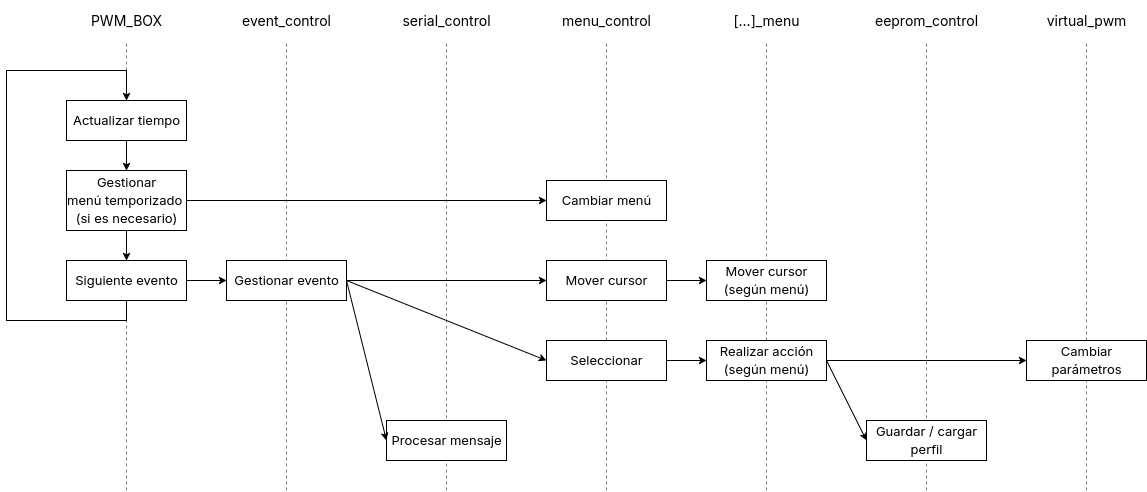
\includegraphics[width=\paperwidth,angle=-90,origin=c]{fw_loop.png}
    \caption{Ejecución del bucle principal.}
    \label{fig:fw_loop}
\end{figure}

\begin{figure}
    \centering
    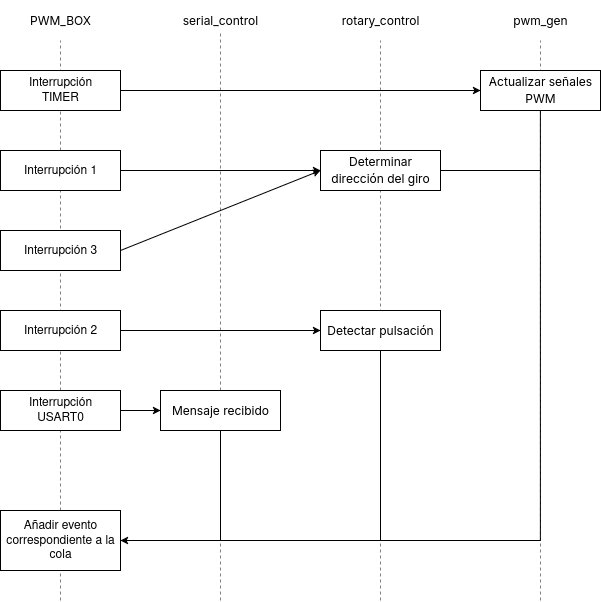
\includegraphics[width=\textwidth]{fw_interrupts.png}
    \caption{Ejecución de las distintas interrupciones.}
    \label{fig:fw_interrupts}
\end{figure}

\section{Desarrollo}

En esta sección se detallarán las decisiones enfrentadas durante la implementación del firmware, centrándose en los cambios propuestos. Para comentarlos más fácilmente, se dividirá la sección en distintas partes, tratando cada funcionalidad añadida por separado.

Antes de entrar en los cambios concretos, cabe destacar que también se ha realizado una extensa labor de limpieza del código, debido a una gran cantidad de funciones y variables sin usar, funciones redundantes y algunas prácticas que no se consideraban óptimas. En muchos casos, el código ha sido prácticamente reimplementando. No se pretende hacer referencia constante a ello, pero no mencionarlo sería subestimar el trabajo realizado en esta parte del proyecto.

\subsection{Memoria EEPROM}

En un primer lugar, se definieron los siguientes tipos de datos:

\begin{itemize}
    \item\textbf{pwm\_t:} Representa una señal PWM en la memoria. Para ello, se almacenan los 4 parámetros principales de la señal (modo, frecuencia, ciclo y fase) junto a su nombre.
    \item\textbf{slot\_t:} Representa el contenido de una ranura de memoria, siendo esta la unidad principal con la que trabajará la memoria. Consiste de 8 señales PWM y de un nombre. Se añadirá, además, una variable que indicará si la ranura está ocupada o no. Esto permitirá evitar borrados reales de memoria, prolongando su vida útil y disminuyendo el coste en rendimiento de la escritura.
\end{itemize}

Otros parámetros que se necesitarán guardar son:

\begin{itemize}
    \item\textbf{Valor de inicialización:} Servirá para determinar si la memoria contiene o no datos, ya que en caso de que no los contenga, necesitará ser inicializada.
    \item\textbf{Número de serie:} Identificador del dispositivo.
    \item\textbf{Contraseña:} Contraseña establecida en el dispositivo. Se guardará como un literal, que no es una buena práctica, pero no se considera necesario seguridad adicional considerando el público objetivo.
    \item\textbf{Ranura por defecto:} Indica la ranura de memoria que se cargará automáticamente al iniciar el PWM Box.
    \item\textbf{Brillo de la pantalla:} Permitirá mantener el brillo establecido entre ejecuciones.
\end{itemize}

A estos se une un vector auxiliar, que incluye el índice de las ranuras reales en el orden en el que se le muestra al usuario en el menú principal. Actúa, por así decirlo, como un traductor entre el índice de las ranuras visibles al usuario y el índice de las mismas internamente. Esto puede entenderse más fácilmente con una representación, que se incluye en la \autoref{fig:eeprom_operations}



Con todo esto, el contenido de la memoria EEPROM puede verse en la \autoref{fig:eeprom_vars}.

\begin{figure}
    \centering
    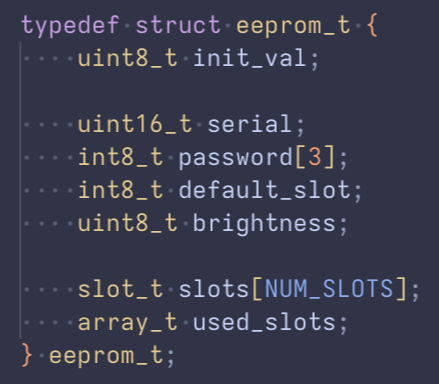
\includegraphics[width=0.5\textwidth]{eeprom_vars.png}
    \caption{Contenido de la memoria EEPROM.}
    \label{fig:eeprom_vars}
\end{figure}

El uso de la directiva \verb|EEMEM|, de la librería \verb|avr/eeprom.h|, permite declarar variables en la memoria EEPROM. Estas, sin embargo, solo servirán para almacenar la dirección de memoria en la que se encuentran los datos. Para leerlos o escribirlos, es necesario usar las funciones proporcionadas por esa misma librería. Por ello, la mayoría de funciones incluídas en esta parte no son más que distintos \textit{getters} y \textit{setters} para las distintas variables mencionadas.

\subsection{Rotary control}

En este apartado, el objetivo principal era el de corregir el funcionamiento algo errático del \textit{rotary encoder}. Sin embargo, la lógica del código presente no estaba del todo clara, por lo que se acabó reimplementando todo de cero.

Para la manipulación de puertos del microcontrolador, se usó por supuesto el manual del ATMega 2560\footnote{Descargable desde el siguiente enlace: \url{https://ww1.microchip.com/downloads/aemDocuments/documents/OTH/ProductDocuments/DataSheets/ATmega640-1280-1281-2560-2561-Datasheet-DS40002211A.pdf}}.

% TODO: Incluir imagen en la que se vea qué es un cambio de flanco (o algo así)

\paragraph{Pulsaciones.} El microcontrolador está programado para generar una interrupción en cada cambio de flanco. Esto, en el caso del botón, significa que se generará una interrupción al pulsarse y otra al soltarse. En cada una, habrá por lo tanto que comprobar el estado del botón en ese instante. En caso de que se encuentre pulsado, se guardará en una variable ese instante de tiempo. Si por el contrario no está pulsado, se comparará la variable anterior con el instante actual (momento en el que termina la pulsación). De esta forma, se determina si el botón se ha pulsado o si se ha mantenido. Este será el resultado de la operación, cuyo evento correspondiente se añadirá al buffer.

A esto se le añade una pequeña lógica de \textit{debouncing}, que sólo tendrá en cuenta cada pulsación si la anterior se ha realizado fuera de una breve ventana de tiempo. Esto evita detectar pulsaciones duplicadas debido a inexactitudes en el circuito del codificador.

\paragraph{Giros.} La lógica para el giro del \textit{rotary encoder} es más compleja. Debido al funcionamiento del mismo, la dirección de giro se puede determinar según el orden en el que dos pines reciban voltaje. De esta forma, se puede crear una máquina de estados para comprobar la dirección del giro según ambos pines vayan o no transmitiendo corriente.

Para ello, también se programa el microcontrolador para que emita una interrupción en ambos flancos de ambos pines, y se va comparando su estado con el de la máquina de estados mencionada. Este funcionamiento se ha encontrado en la librería \url{https://github.com/buxtronix/arduino/tree/master/libraries/Rotary}, cuyo código fuente ha sido adaptado para funcionar en este proyecto.

% Un rotary encoder consiste de un disco giratorio sobre el que se distribuyen unas zonas de contacto. El disco suele conectarse a tierra, mientras que las zonas de contacto servirán para transmitir voltaje. Al girar el rotary encoder, ambos pines A y B harán contacto con una de las zonas brevemente, generándose un pulso representable como una señal cuadrada. 

\subsection{Serial control}

Para la comunicación por el puerto serie también ha sido necesario manipular los puertos del microcontrolador. Para ello, se han habilitado las interrupciones RX (para la recepción) y TX (para el envío) y se ha configurado la comunicación para usar 8-bits por segmento. En cuanto a la velocidad de transmisión, se ha activado la \textit{Double Speed Operation} del ATMega 2560 para llegar a los 115200 baudios.

En cuanto a implementación se han programado, en primer lugar, funciones básicas para el envío y recepción de datos. Posteriormente, se han usado las mismas para implementar el sistema de envío y recepcion de datos, ya cubiertos en % TODO


\subsection{Sistema}
\subsection{Común}
\subsection{PWM}


\section{Pruebas}

